\lesson{Rate Equations and Order of Reactions}
Experimental evidence suggests that the rate of a reaction is exponentially proportional to 
the product of the initial concentrations of the reactants. That is, in a balanced chemical equation
\[
    aX+bY\to \text{products}
\]
The rate law states that
\begin{align*}
    r&\propto [X]^m[Y]^n\\
     &=k[X]^m[Y]^n
\end{align*}
Where $m$ and $n$ describe the relationship between initial concentration and rate, determined
emrpically. $k$ is the rate constant, which is determined in several different units, depending
on the \textbf{overall order of the reactants}. The \textbf{order of reaction} is the exponent value
that describes the initial concentration dependence of a particular reactant.

\newpage
\begin{figure}[ht!]
    \centering
    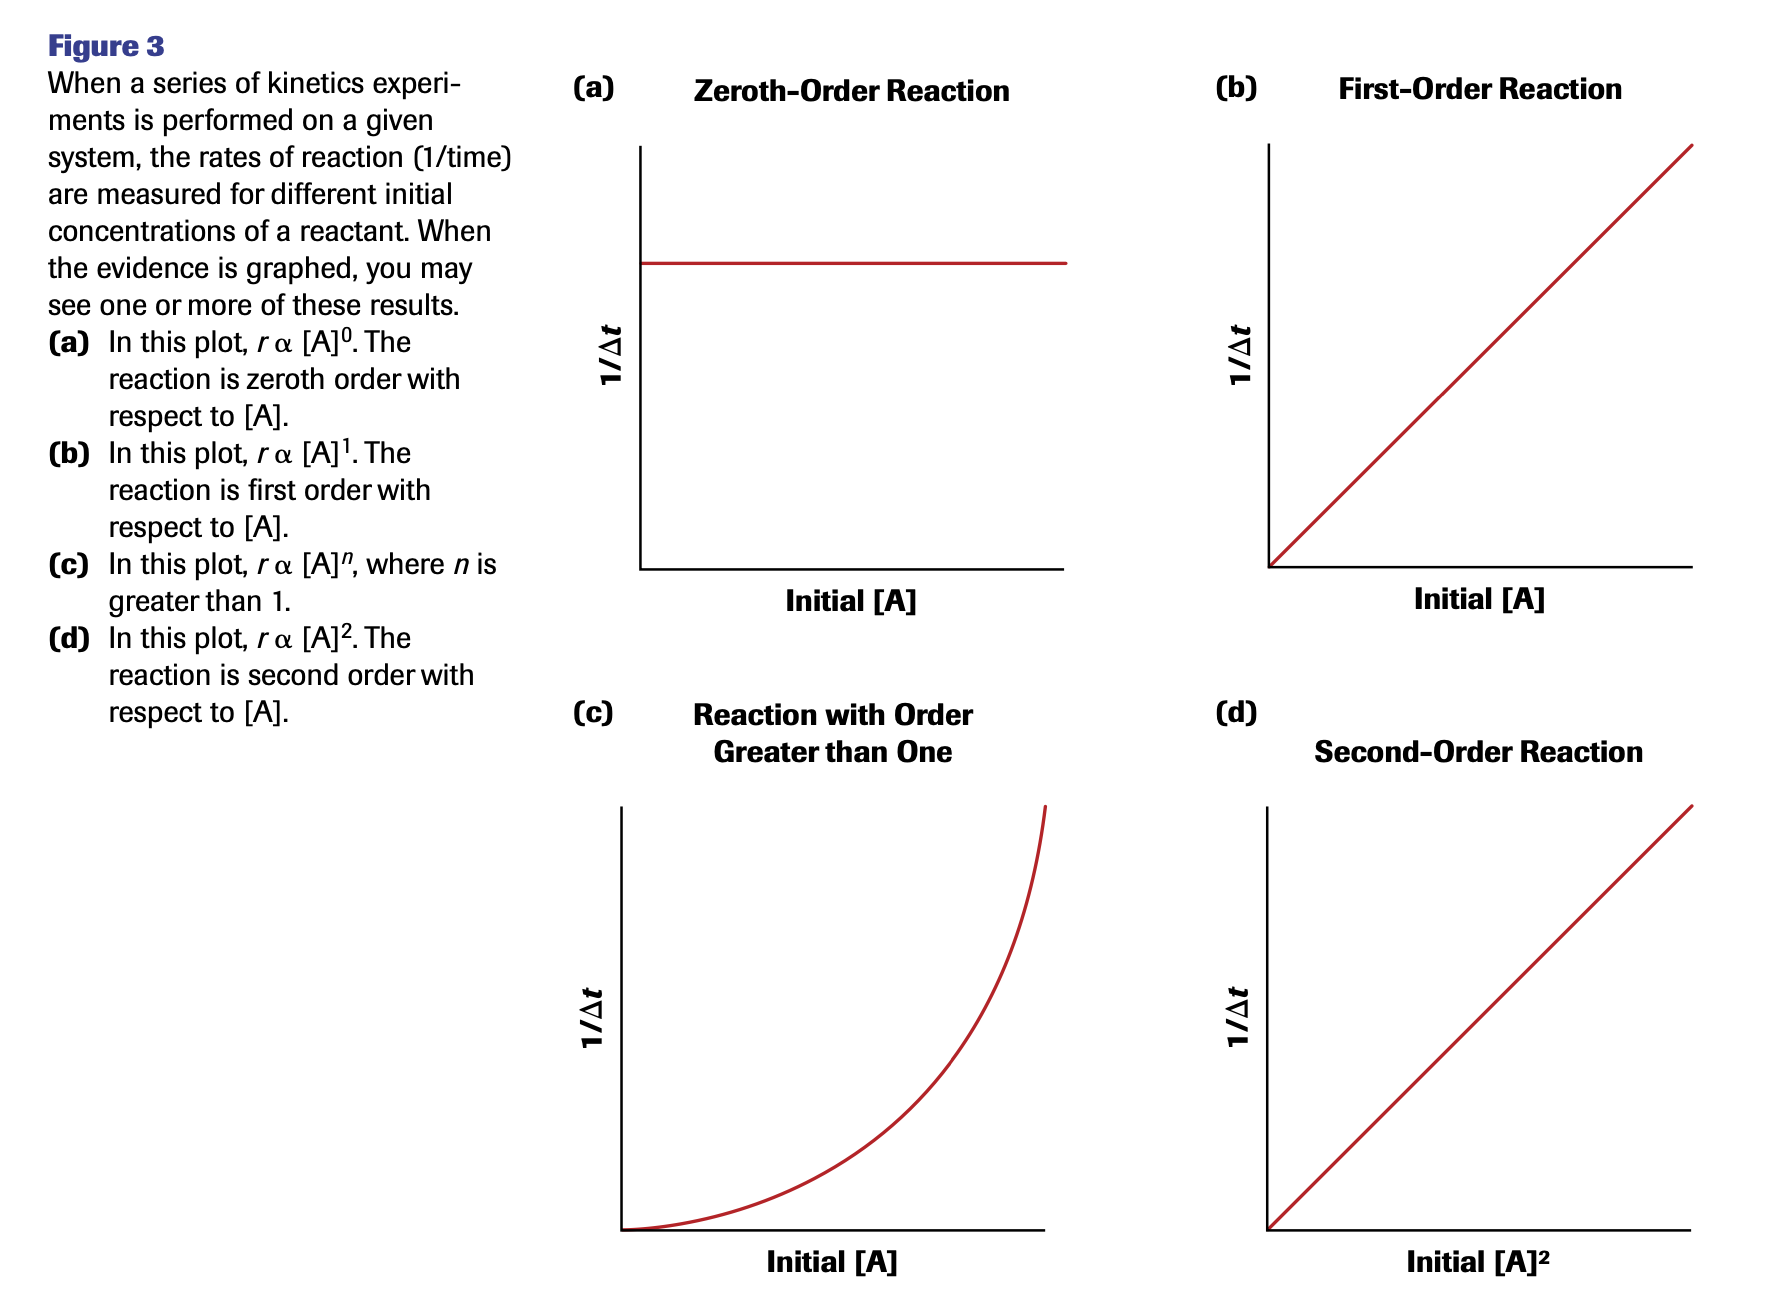
\includegraphics[width=\textwidth]{../figures/order of reaction.png}
    \caption{Note that (d) is most likely wrong. It should be curved.}
\end{figure}

\begin{sample}{Consider the data in the table below and calculate the overall order of the reaction.
        And the rate constant.
        \begin{tabular-custom}{|c|c|c|c|}{}
            Trial & [A] (mol/L) & [B] (mol/L) & Rate (mol/(Ls)) \\ \hline
            1 & 1.0 & 2.0 & 0.523 \\ \hline
            2 & 5.0 & 2.0 & 2.610 \\ \hline
            3 & 1.0 & 3.0 & 1.177 \\ \hline
        \end{tabular-custom}
    }
    Analyzing the trials for [A]
    \begin{align*}
        (\frac{5.0}{1.0})^y=\frac{2.610}{0.523}\\
        5^y&=4.99043977\\
        y&=1
    \end{align*}
    Therefore, [A] is a order 1 reactant. Analyzing the trials for [B]
    \begin{align*}
        (\frac{3.0}{2.0})^y&=\frac{1.177}{0.523}\\
        (1.5)^y&=2.25047801\\
        y&=2
    \end{align*}
    Therefore, [B] is a order 2 reactant. Plugging in these values for $k$
    \begin{align*}
        k&=\frac{r}{[A][B]^2}\\
         &=\frac{2.610\,\si{mol.L^{-1}.s^{-1}}}{(5.0\,\si{mol.L^{-1}})(2.0\,\si{mol.L^{-1}})^2}\\
         &=0.1305\,\si{mol^{-1}L^2s^{-1}}
    \end{align*}
\end{sample}

\begin{important}
    A particular common type of first degree reaction is a \textbf{decomposition reaction}. 
    Specifically, \textbf{radioactive decay} is a first order reaction. 
\end{important}
